\newpage
\section{CouchDB}
Apache \ac{CouchDB} è \ac{DBMS} 
non relazionale ottimizzato per essere utilizzato in applicazioni web. È un
database opensource, nato nel 2005 e mira a diventare il database di Internet.

\ac{CouchDB}, essendo un database \ac{NoSQL}, memorizza i dati come documenti
utilizzando il formato \ac{JSON}.
Ogni database è una collezione di documenti ed ogni documento contiene i propri
dati e schema in modo indipendente dagli altri. Il documento memorizzato in una
base di dati contiene tutte le proprietà dell'oggetto che si vuole rappresentare
e, inoltre, memorizza i metadata associati ad esso :
\emph{``\_id"} e \emph{``\_rev"}. La variabile \emph{``\_id"} rappresenta l'id univoco
per ogni documento e, se non viene istanziata dall'utente, assume un valore assegnato
dal motore di CouchDB.
La propretà \emph{``\_rev"} viene utilizzata per la gestione delle revisioni.
\ac{CouchDB} è in grado di gestire la contemporaneità di accesso ad una risorsa
fra un elevato numero accessi in lettura e scrittura della risorsa stessa. Questo
sistema è implementato tramite \ac{MCC}.

Proviamo ad immaginare il caso in cui un utente prova a leggere una risorsa e
nello stesso istante un secondo utente la sta usando e modificando. Se questo
passaggio critico non viene gestito in modo corretto, è possibile che il lettore
veda la risorsa in modo inconsistente, in uno stato non completo e con una
perdita parziale o totale dei dati. Questo tipo di situazione può, inoltre,
creare stalli ed errori nell'applicazione che accede alla risorsa.
Una soluzione per evitare ciò, è quella di bloccare la risorsa appena un utente
prova accedere per modificarla. Limitare la risorsa ad un accesso contemporaneo
non sempre è accettabile, in quanto blocca tutte operazioni di lettura e
scrittura, rendendo inaccessibile la risorsa.

\ac{MCC} propone un approccio differente : ogni utente che accede alla risorsa,
ne visualizza il suo ultimo stato consistente, cioè uno stato in cui tutti ivincoli
definiti dalla risorsa sono rispettati. In questo modo le modifiche effettuate
da un utente non saranno visibili fino a che non viene completata l'operazione
di scrittura. Tutti gli utenti, però, potranno accedere contemporaneamente alla
risorsa. Per permettere ciò, ad ogni modifica non viene aggiornato direttamente
il documento restituito dalla richiesta, ma lo si segna come obsoleto e se ne
crea uno nuovo aggiornato, al quale verrà assegnato un nuovo valore della
versione. La chiave \emph{``\_rev''} viene, dunque, aggiornata e questo
meccanismo è alla base della prevenzione dei conflitti in fase di salvataggio.
In questo modo ci sono più versioni dell'oggetto, ma solo una di esse è l'ultima
versione. Per evitare sovraccarichi di documenti obsoleti è necessario che il
sistema periodicamente faccia pulizia e cancelli i dati più vecchi. CouchDB
predispone di un sistema di \emph{merging} dei documenti per non perdere le
modifiche fatte da diversi utenti alla stessa risorsa.
\\\\
\ac{CouchDB} fornisce la semantica \ac{ACID} per tutte le transazioni. Una transazione è una sequenza
di operazioni che può concludersi con un successo o un fallimento. In caso di
successo il risultato delle operazioni deve essere permanente, mentre in caso
di insuccesso si deve tornare allo stato della risorsa che aveva al
momento dell'inizio della transazione. Aderire alla semantica \ac{ACID},
permette di avere un sistema stabile e che mantiene il corretto funzionamento,
anche a fronte di errori esterni, come ad esempio un mancanza della connessione
durante l'invio dei dati, o crash del sistema.
Di seguito l'analisi delle proprietà \acf{ACID}~:
\begin{itemize}
  \item \textbf{Atomicity}: la transazione è indivisibile nella sua esecuzione e
  la sua esecuzione deve essere o totale o nulla, non sono ammesse esecuzioni
  parziali. In caso di fallimento dell'operazione si ritorna allo stato
  precedente;
  \item \textbf{Consistency}: la transazione porta l'oggetto sul quale si opera
  da uno stato consistente iniziale ad un secondo stato consistente finale.
  La transazione non deve violare eventuali vincoli di integrità, quindi non 
  devono verificarsi contraddizioni tra i dati archiviati nel database;
  \item \textbf{Isolation}: ogni transazione deve essere eseguita in modo
  isolato e indipendente dalle altre transazioni. L'eventuale fallimento di una
  transazione non deve interferire con le altre transazioni in esecuzione;  
  \item \textbf{Durability}: detta anche persistenza, garantisce che una
  transazione eseguita rimarrà valida anche in caso di errori successivi. I
  cambiamenti apportati non dovranno essere persi per crush o errori nel
  sistema. Per evitare che nel lasso di tempo fra il momento in cui la base di
  dati si prepara a scrivere le modifiche e quello in cui li scrive
  effettivamente si verifichino perdite di dati dovuti a malfunzionamenti, le
  operazioni eseguite verranno registrate su file di log.
\end{itemize}

\newpage
\subsection{JSON}
I \ac{DBMS} orientati ai documenti non memorizzano i dati in struttura tabelle
con campi prefissati per ogni record come nei database relazionali, ma ogni valore è
memorizzato come un documento con determinate caratteristiche. Qualsiasi numero
di campi e qualsiasi tipologia di dato rappresentato può essere aggiunto al
documento.
\\\acf{JSON} è un formato basato sul linguaggio
\emph{Javascript} utilizzato per lo scambio d'infomazioni in applicazioni
client-server e utilizzato come formato da alcuni DBMS orientati ai documenti,
quali \ac{CouchDB} o MongoDB.
Attraverso la notazione \ac{JSON} è possibile rappresentare qualsiasi proprietà
di un oggetto, con il vantaggio che la struttura del documento non è vincolata ad un
modello prefissato, ma può variare nel tempo. Infatti è possibile aggiungere e
rimuovere proprietà dell'oggetto o addirittura modificarne il tipo di dato
rappresentato ed è possibile inserire attributi multipli o oggetti.
\\\\Un documento \acl{JSON} è formato da due strutture:
\begin{itemize}
  \item Una collezione di coppie ``nome''/``valore'' ;
  \item Un elenco ordinato di valori. 
\end{itemize}
Un oggetto è una collezone non ordinata di coppie ``nome'' : ``valore''. Un
oggetto inizia con una parentesi graffa aperta ``\{`` e finisce con una parentesi
graffa chiusa ~`\}''. Un oggetto può essere asseganto
come valore ad una variabile~(Figura~\ref{fig:jsondoc}).
 \begin{figure}[!h]
  \begin{center}
      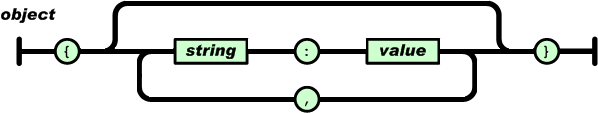
\includegraphics[scale=0.50]{icons/jsondoc.png}
      \caption{Oggetto JSON}
      \label{fig:jsondoc}
  \end{center}
\end{figure}
\\Un array è un insieme ordinato di valori. Un array comincia con una
parentesi quadra sinistra ``{[}'' e finisce con una parentesi destra``{]}''. I
valori sono separati da una~virgola~``,''~(Figura~\ref{fig:jsonarray}).
\begin{figure}[!h]
\begin{center}
    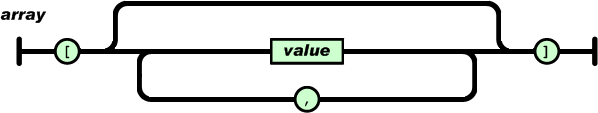
\includegraphics[scale=0.50]{icons/jsonarray.png}
    \caption{Array JSON}
    \label{fig:jsonarray}
\end{center}
Ogni nome di variabile è seguito dai due punti ``:'' e le coppie
``nome'' : ``valore'' sono separati
da una~virgola~``,''~(Figura~\ref{fig:jsonvalue}). In CouchDB assumono
significato particolare le variabili ``\_id'' e ``\_rev''. 

\end{figure}
\begin{figure}[!h]
  \begin{center}
      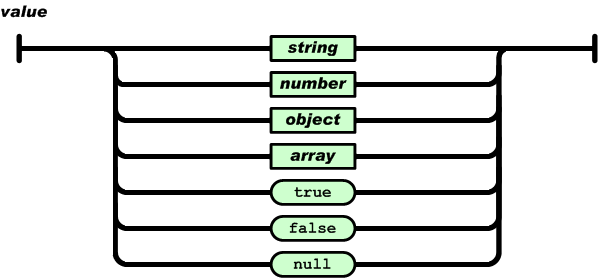
\includegraphics[scale=0.50]{icons/jsonvalue.png}
      \caption{Valore di una variabile JSON}
      \label{fig:jsonvalue}
  \end{center}
\end{figure}

\\L'oggeto utilizzato nel nostro modello è composto da sei variabili.
\emph{department} indica la facoltà per la quale è stata registrata una
votazione, il valore è una stringa univoca, nel caso la votazione si
riferisca ad un'operazione eseguita presso lo sportello veloce verrà registrata
con \emph{``sportello''}.\emph{Score} è una variabile numerica intera , nel
nostro modello può assumere i valori \{1,3,5\}.La data di effettuazione della
votazione,\emph{date} , viene raccolta dal sistema e salvata nel formato
``Y-m-d''.Gli attributi \emph{comment},\emph{customerName} e
\emph{customerEmail} nel caso il ciente lasci un feedback sono di tipo stringa , \emph{null} altrimenti. 
\\
\begin{lstlisting}[language=json] 
{ 
   _id:"182b00cd54a2b054fffabf1042000fbb", 
   _rev:"1-cb887f197900dce789c2dca898e4d330", 
   agency: "vicenza",
   operation: "counter",
   score: 5,
   date: "2013-06-01T11:40:52.280Z",
   comment: "Servizio efficiente",
   customerName: "Alex Tomasello",
   customerEmail: null
}
\end{lstlisting} 

\newpage
\subsection{API}
Il database è accessibile tramite richieste \acf{HTTP}, le cui proprietà sono
specificate nella \ac{RFC} 2616. Una richiesta
\ac{HTTP} è formata da una riga di richiesta (\emph{request line}) che contiene
il metodo, lo \ac{URI} e la versione del protocollo. La seconda componente della
richiesta è la sezione \emph{header} , la terza il \emph{body}. 

Attraverso i metodi messi a disposizione dal protollo,
è possibile memorizzare nuovi dati e creare nuove viste (\emph{Create}),
richiedere informazioni (\emph{Read}), modificare le informazioni memorizzate
all'interno dei documenti (\emph{Update}) ed eliminare documenti
(\emph{Delete}).

Ogni documento è raggiungibile da uno \ac{URL} univoco. Il protocollo \ac{HTTP}
prevede la seguente sintassi per definire l'~\ac{URL} di una risorsa alloccata : 

http\_URL = ``http:'' ``//'' host [ ``:'' port ] [ abs\_path [ ``?'' query
]]
\\
\emph{Host} è l'indirizzo del server sul quale è ospitato il database,
\emph{port} indica la porta sulla quale è in ascolto CouchDB, che di default è
la 5984 per richieste http, 6984 per ssl, modificabili accedendo al file di
configurazione. Se si vuole accedere al database \emph{abs\_path} è il nome del
database stesso, se si vuole accedere ad una vista il percorso da inserire sarà
composto da

nome\_database ``/\_design/'' nome\_design\_document ``/\_view/'' nome\_vista.
\\\\
Le operazioni \ac{CRUD}  sulle risorse sono
eseguibili tramite i seguenti metodi \ac{HTTP} ( gli esempi riportati sono stati
realizzati con il command line tool \textit{cURL}):
\begin{itemize}
  \item \textbf{GET} : richiede l'elemento specificato. Il formato dell'\ac{URL}
  definisce ciò che viene restituito: CouchDB può restituire elementi
  statici (ad esmepio viste), documenti di database e di configurazione.
  L'informazione viene restituita sotto forma di un documento \ac{JSON}.
  Per ottenere documenti non l'URL deve essere composto da :
  
  ``http://'' host ``:'' port ``/'' database ``/'' \_id
  
  es: \emph{curl -X GET ``http://atcustomersat:5984/padova/55090\ldots''}.
  
  Per ottenere elementi statici come le viste l'URL deve essere composto da:
  
  ``http://'' host ``:'' port  ``/'' database ``/\_design/''\_id 
  
  es: \emph{curl -X GET
  ``http://atcustomersat:5984/padova/\_design/consulting''}.
  
  \item \textbf{HEAD} : questo metodo viene utilizzato per ottenere
  l'intestazione \ac{HTTP} di una richiesta GET senza il corpo della risposta.
  Viene utilizzato per verificare l'esistenza di un oggetto senza richiederne il
  contenuto. In caso di documenti di grandi dimensioni, verificarne l'esistenza
  con il metodo HEAD velocizza notevolmente l'applicazione, in quanto non si
  deve aspettare che ritorni l'oggetto richiesto. L'\ac{URL} per accedere ai
  documenti ha la stessa sintassi di una richiesta GET.
   
  es: \emph{curl -X HEAD ``http://atcustomersat:5984/padova/55090\ldots''}
  \item \textbf{POST} : permette di inviare nuovi documenti al database di
  destinazione. In questo caso la richiesta POST deve avere come
  contenuto del body un documento \ac{JSON} valido.
  
  Per inviare un documento l'URL deve essere composto da:
  
  ``http://'' host ``:'' port ``/'' database 
  
  es : \emph{curl -X POST ``http://atcustomersat:5984/padova'' -H
  ``Content-Type:}
  \emph{application/json'' --data @scorecard.json}
  
  Dove \emph{scorecard.json} è un file contentente un documento json. 
  \item \textbf{PUT} : permette di inviare una risorsa specificata. In
  CouchDB il metodo PUT può essere utilizzato per creare nuovi dodumenti e
  database.
  
  es : \emph{curl -X PUT ``http://atcustomersat:5984/padova/123456798''}
  \emph{ -H ``Content-Type:application/json'' --data @scorecard.json}
  \item \textbf{DELETE} : cancella la risorsa specificata.
  
  es: \emph{curl -X DELETE ``http://atcustomersat:5984/padova/55090\ldots''}
\end{itemize}
Per aderire alle specifiche HTTP, è necessario, inoltre, che gli headers
siano settati e vengano forniti in modo da ottenere il formato e codifica
corretta. Gli headers essenziali sono \emph{Content~-~type} e \emph{Accept}.
\textbf{Content~-~type} specifica il tipo di contenuto dei dati che
vengono forniti nella richiesta. CouchDB accetta il formato JSON quindi l'header
sarà \emph{application/json}.
L'header \textbf{Accept}, invece, indica quali tipi di file sono accettati dal
client, in formato MIME (es: text/html). Solitamente sarà settato con
\emph{application/json}, \emph{*/*} se sono supportati tutti i tipi di file.
\\\\
Per realizzare interrogazioni parametrizzate, si usano le query-string. La
query-string è la parte di un URL che contiene dei dati da passare in input ad
un programma. Il carattere ``?'' apre la query-string, è utilizzato come
carattere speciale e non viene incluso nella query. Ogni argomento è formato da
una coppia chiave - valore. Alla chiave X si assegna il valore Y con il segno
``='' ed ogni argomento è separato da un altro con il carattere ``\&''. 
La sinstassi per realizzare una query string è, dunque, la seguente :

  
``?parametro1=valore1\&parametro2=valore2\&parametro3=valore3''.
\\\\
Le query parametrizzate vengono utilizzate nell'applicazione nel momento della
generazione dei grafici. C'è la possibilità di scegliere la sede che si vuole
monitorare, il tipo di servizio, l'intervallo temporale e il tipo di grafico.
Ogni voce scelta andrà a settare un parametro nell'\ac{URL}. I parametri
permessi da CouchDB sono illustrati nella tabella seguente.
\\\\
\begin{tabular}{|>{\columncolor{background}}p{2.4cm}|p{3.1cm}|p{1.4cm}|p{5.8cm}|}
  \hline
  \rowcolor{table}
  \textbf{Parametro} & 
  \textbf{Valore} & 
  \textbf{Default} &
  \textbf{Descrizione}
   
  \\\hline key & JSON & - & Indica la coppia chiave-valore, deve rispettare
  la sintassi dell'URL.
  \\\hline startkey & JSON
    & - & Indica il valore della chiave di partenza, deve rispettare la
    sintassi dell'URL.
  \\\hline startkey\_docid & ``\_id'' del documento & - & ID del documento di
  partenza.
  \\\hline endkey & JSON
    & - & Indica il valore massimo della chiave, deve rispettare la
    sintassi dell'URL.
  \\\hline endkey\_docid & ``\_id'' del documento & - & ID del documento che
    termina la ricerca.
  \\\hline limit & intero & - & Limita il numero di documenti
    restituiri.
  \\\hline descending & true/false & false & Ordinamento della ricerca.
  \\\hline skip & intero & 0 & Salta il numero indicato di documenti.
  \\\hline group & true/false & false & Controlla se la funzione di
    \emph{reduce} viene applicata a un gruppo di chiavi distinte o singola riga di
    risultati.
  \\\hline group\_level & intero & - & Indica il livello di raggruppamento da
  applicare alla funzione \emph{reduce}.
  \\\hline reduce & trey/false & true & Specifica se utilizzare la funzione
  \emph{reduce}.
  \\\hline
\end{tabular}
\\\\
Ad esempio per ricevere i dati di una particolare sede, ragguppati per mesi e
per il periodo temporale compreso tra gennaio e luglio 2013, la query è la
seguente

?group\_level=2\&startkey=[2013,1,1,1]\&endkey=[2013,7,31,23]
\newpage
\subsection{Replication} 
CouchDB consente si sincronizzare database situati su differenti host
permettendo quindi agli utenti di accedere a risorse situate su host diversi in
modo trasparente.
La sincronizzazione è possibile perchè CouchDB è un database
NOSQL e quindi ogni base di dati è una collezione di documenti indipendenti tra
di loro, cioè che documenti diversi possono rappresentare oggetti
diversi.
La sincronizzazione è unilaterale, bisogna indicare un server che conterrà
il database originale (\emph{source}) e uno con funzione di \emph{target}.
Un database viene definito ``locale'' quando si trova sulla stessa istanza del
server al quale viene inviata la richiesta di replication.
Tutti gli altri casi i database sono definiti ``remoti''.
Per sincronizzare un database si effettua una richiesta POST, inviando nel body
un documento JSON contenente i database di source e destination:

\begin{lstlisting}[language=json]
//file replication.json:
{
  source:"database",
  target:"http://example.org/database"
}
\end{lstlisting}
 
 
\emph{curl -X POST http://atcustomersat:5984/\_replicate -H ``Content-Type:}
\emph{application/json'' --data @replication.json}
\\\\
Quando si utilizza la sincronizzazione, CouchDB confronta i due database e
verifica quali documenti presenti nel source differiscono da quelli presenti nel
target. I documenti alloccati nel target verranno modificati , cancellati o
creati a seconda dello stato di quelli presenti nell'origine. Il numero di
revisione del documento viene modificato, ed è possibile risalire alle modifiche
effettuate al momento della sincronizzazione. Per realizzare una
sincronizzazione bilaterale basta inviare due richieste di replication
invertendo target e source.

Aggiungendo il parametro continuous e settandolo a true, è possibile continuare
a sincronizzare i database ogni volta che vengono aggiunti o modificati
documenti nel database di source. Nell'attuale versione di CouchDB ( v1.3.0) non
è possibile continuare la sincronizzazione dopo il riavvio del server, in quanto
i settaggi della replication vengono resettati.

\newpage
\subsection{Map-Reduce}
\emph{MapReduce} è un framework software per scrivere facilmente applicazioni
che elaborano grandi quantità di dati in parallelo. Il sistema è formato da due
funzioni~: \emph{map} e \emph{reduce}. La prima elabora le coppie chiave-valore
, la seconda elabora il set di coppie generate dalla funzione \emph{map} 
restituendo l'output richiesto.
\begin{itemize}
  \item \emph{map}: il nodo master prende i dati di ingresso (fase
  \emph{input}), li suddivide in piccoli blocchifase
  \emph{splitting}, generalmente da 64MB o 128MB e distribuisce il lavoro ai
  nodi slaves. Il singolo nodo \emph{mapper} produce il risultato intermedio della
  funzione di map() sotto forma di coppie [chiave,valore] memorizzate su un file
  distribuito, la cui locazione è notificata al master alla fine della fase di
  map (fase \emph{mapping}).
  \item \emph{reduce}: il nodo master colleziona le risposte, combina le coppie
  [chiave,valore] in liste di valori che condividono la stessa chiave e li
  ordina per chiave (fase
  \emph{shuffling}). Le coppie della forma,
  [chiave,IteratorList(valore,\ldots)] sono passate ai nodi reducer che
  eseguono la funzione di reduce() (fase
  \emph{reducing}).
\end{itemize}
Le funzioni di \emph{map} e \emph{reduce} sono implementate in Javascript, e
CouchDB mette a disposizione ulteriori funzioni native da utilizzare.
La funzione \emph{reduce} come parametri di input ha una collection di chiavi,
una collection di valori e un valore booleano \emph{rereduce}. Se settato a
true, rereduce permette di usare la funzione reduce al blocco di risultati
generato dalle chiamate della funzione. Per database di grandi dimensioni,
CouchDB chiama le funzioni per blocchi di dati in modo da velocizzare l'analisi
dei dati. Non applicando la funzione rereduce c'è il rischio di ottenere un
output sbagliato.

 Ad esempio ipotizziamo di avere un set di documenti
composto da 1000 chiavi.
La fase di map calcola ``chiave''=``valore'' e il motore di CouchDB divide i
documenti ricevuti come input in 3 blocchi. Nella fase di reduce, la funzione
calcola quanti elementi sono presenti nel db. La situazione di partenza prevede
1000 oggetti, la fase di map e reduce divide in 3 blocchi contenenti
rispettivamente 333,333 e 334 oggetti.
L'output resituito dalla funzione reduce è errato, in quanto calcola il numero
di oggetti presenti restituito dopo le operazioni, calcola quindi 3
oggetti(~Figura~\ref{fig:reduce}).
Applicando la funzione di rereduce, invece, viene calcolata la somma dei valori
restituiti dai 3 oggetti temporanei, restituendo l'output
corretto(~Figura~\ref{fig:rereduce}).


\begin{figure}[!h]
\begin{tikzpicture}[%
  >=triangle 60,              % Nice arrows; your taste may be different
  start chain=going below,    % General flow is top-to-bottom
  node distance=6mm and 60mm, % Global setup of box spacing
  every join/.style={norm},   % Default linetype for connecting boxes
  ]
\tikzset{
  base/.style={draw, on chain, on grid, align=center, minimum height=4ex},
  proc/.style={base, rectangle, text width=10em},
  map/.style={base, rectangle, text width=10em},
  cong/.style={->, draw, lccong}, 
  it/.style={font={\small\itshape}}
}
\node
[proc,xshift=12em](input){\textbf{key}~,~\textbf{val}\\1~,~1\\\ldots~,\ldots\\1000~,~5984};
\node [proc,xshift=-12em](split1){\textbf{key}~,~\textbf{val}\\1~,~1\\\ldots~,
\ldots\\333,210};
\node [map,fill=background](map1){function(key,val)~\{\\ count(val);\}};
\node [proc](result1){\textbf{key} , \textbf{val}\\ null~,~333};
\node [proc,xshift=12em,yshift=15.19em](split2){\textbf{key}
,\textbf{val}\\334~, 458\\\ldots~,~\ldots\\666,131}; 
\node [map,fill=background](map2){function(key,val)~\{\\ count(val);\}}; 
\node [proc](result2){\textbf{key} , \textbf{val}\\ null~,~333}; 
\node [proc,xshift=12em,yshift=15.19em](split3){\textbf{key}
,\textbf{val}\\667~,~125\\\ldots~,\ldots\\1000,5984}; 
\node [map,fill=background](map3){function(key,val)~\{\\ count(val);\}}; 
\node [proc](result3){\textbf{key} ,\textbf{val}\\ null~,~334};
\node [map,fill=background,xshift=-12em](reduce){function(key,val)~\{\\ count(val);\}};
\node [proc](output){\textbf{key} , \textbf{val}\\null~,~3};

\path (input.south) to node [near start, xshift=5em] {}
(split1); \draw [->] (input.south) -- (split1.north);
\path (input.south) to node [near start, xshift=5em] {}
(split2); \draw [->] (input.south) -- (split2.north);
\path (input.south) to node [near start, xshift=5em] {}
(split3); \draw [->] (input.south) -- (split3.north);

\path (split1.south) to node [near start, xshift=5em] {}
(map1); \draw [->] (split1.south) -- (map1.north);
\path (split2.south) to node [near start, xshift=5em] {}
(map2); \draw [->] (split2.south) -- (map2.north);
\path (split3.south) to node [near start, xshift=5em] {}
(map3); \draw [->] (split3.south) -- (map3.north);

\path (map1.south) to node [near start, xshift=5em] {}
(result1); \draw [->] (map1.south) -- (result1.north);
\path (map2.south) to node [near start, xshift=5em] {}
(result2); \draw [->] (map2.south) -- (result2.north);
\path (map3.south) to node [near start, xshift=5em] {}
(result3); \draw [->] (map3.south) -- (result3.north);

\path (result1.south) to node [near start, xshift=5em] {}
(reduce); \draw [->] (result1.south) -- (reduce.north);
\path (result2.south) to node [near start, xshift=5em] {}
(reduce); \draw [->] (result2.south) -- (reduce.north);
\path (result3.south) to node [near start, xshift=5em] {}
(reduce); \draw [->] (result3.south) -- (reduce.north);

\path (reduce.south) to node [near start, xshift=5em] {}
(output); \draw [->] (reduce.south) -- (output.north);

\end{tikzpicture} 
\caption{MapReduce con \emph{rereduce=false}}\label{fig:reduce}
\end{figure}

\def\HS{\hspace{\fontdimen2\font}}

\begin{figure}[!h]
\begin{tikzpicture}[%
    >=triangle 60,              % Nice arrows; your taste may be different
    start chain=going below,    % General flow is top-to-bottom
    node distance=6mm and 60mm, % Global setup of box spacing
    every join/.style={norm},   % Default linetype for connecting boxes
    ]
\tikzset{
  base/.style={draw, on chain, on grid, align=center, minimum height=4ex},
  empty/.style={ on chain, on grid, align=center, minimum height=6ex,text
  width=10em},
  proc/.style={base, rectangle, text width=10em, align=center},
  map/.style={base, rectangle, text width=10em,align=left},
  cong/.style={->, draw, lccong}, 
  it/.style={font={\small\itshape}}
}
\node [empty, densely dotted, it] (empty1) { };
\node [proc, densely dotted, it,xshift=12em] (p0) { splitting \space  \&
\space mapping }; \node [map,fill=background](reduce){function(key,val)~\{\\
if (rereduce)\\ \{\space\space\space sum(val) \} \\ else\\
\{\space\space\space count(val) \};\}}; \node [proc](output){\textbf{key} ,
\textbf{val}\\null~,~1000};

\path (p0.south) to node [near start, xshift=5em] {}
(reduce); \draw [->] (p0.south) -- (reduce.north);

\path (reduce.south) to node [near start, xshift=5em] {}
(output); \draw [->] (reduce.south) -- (output.north);

\end{tikzpicture} 
\caption{MapReduce con \emph{rereduce=true}}\label{fig:rereduce}
\end{figure}



\newpage \newpage
Di seguito è presentata la funzione map utilizzata nel calcolo della somma dei
voti per l'operazione di consulenza. Nel momento della fase di map, vengono scartati
i documenti che non appartengono al gruppo scelto. Successivamente viene creata
la coppia chiave-valore da inviare alla funzione di reduce. La chiave è la data
trasformata in un array, per agevolare il raggruppamento in fase di output.

\begin{lstlisting}[language=JavaScript] 
function(doc) {
  if (doc.operation != 'consulting') 
    return;
  var date = new Date(doc.date);
  emit(
    [date.getFullYear(), 
     (date.getMonth()  +1),
     date.getDate(),
     date.getHours()],
    doc.score); 
}
\end{lstlisting}
La funzione reduce raccoglie i dati, distinguendo i casi in cui rereduce è
settato a true oppure a false.
 \begin{lstlisting}[language=JavaScript]
function (key, values, rereduce) {
  // Reduce function
  var count = 0;
  var sum = 0;
  var i;

  if(!rereduce) {
    // `values` stores actual map output
    for(i = 0; i < values.length; i++) {
      count += 1;
      sum += Number(values[i]);
    }
    return {"count":count, "sum":sum};
  }

  else {
    // `values` stores count/sum objects returned previously.
    for(i = 0; i < values.length; i++) {
      count += values[i].count;
      sum   += values[i].sum;
    }
    return {"count":count, "sum":sum};
  }
}
\end{lstlisting}
